% !TeX root = main.tex
\section{Fundamental Matrix}

\subsection*{Brief Description and Notation}

Please refer to Figure \ref{fig:q1-epipolar-geometry} for the notations and meaning.

\begin{figure}[h]
    \centering
    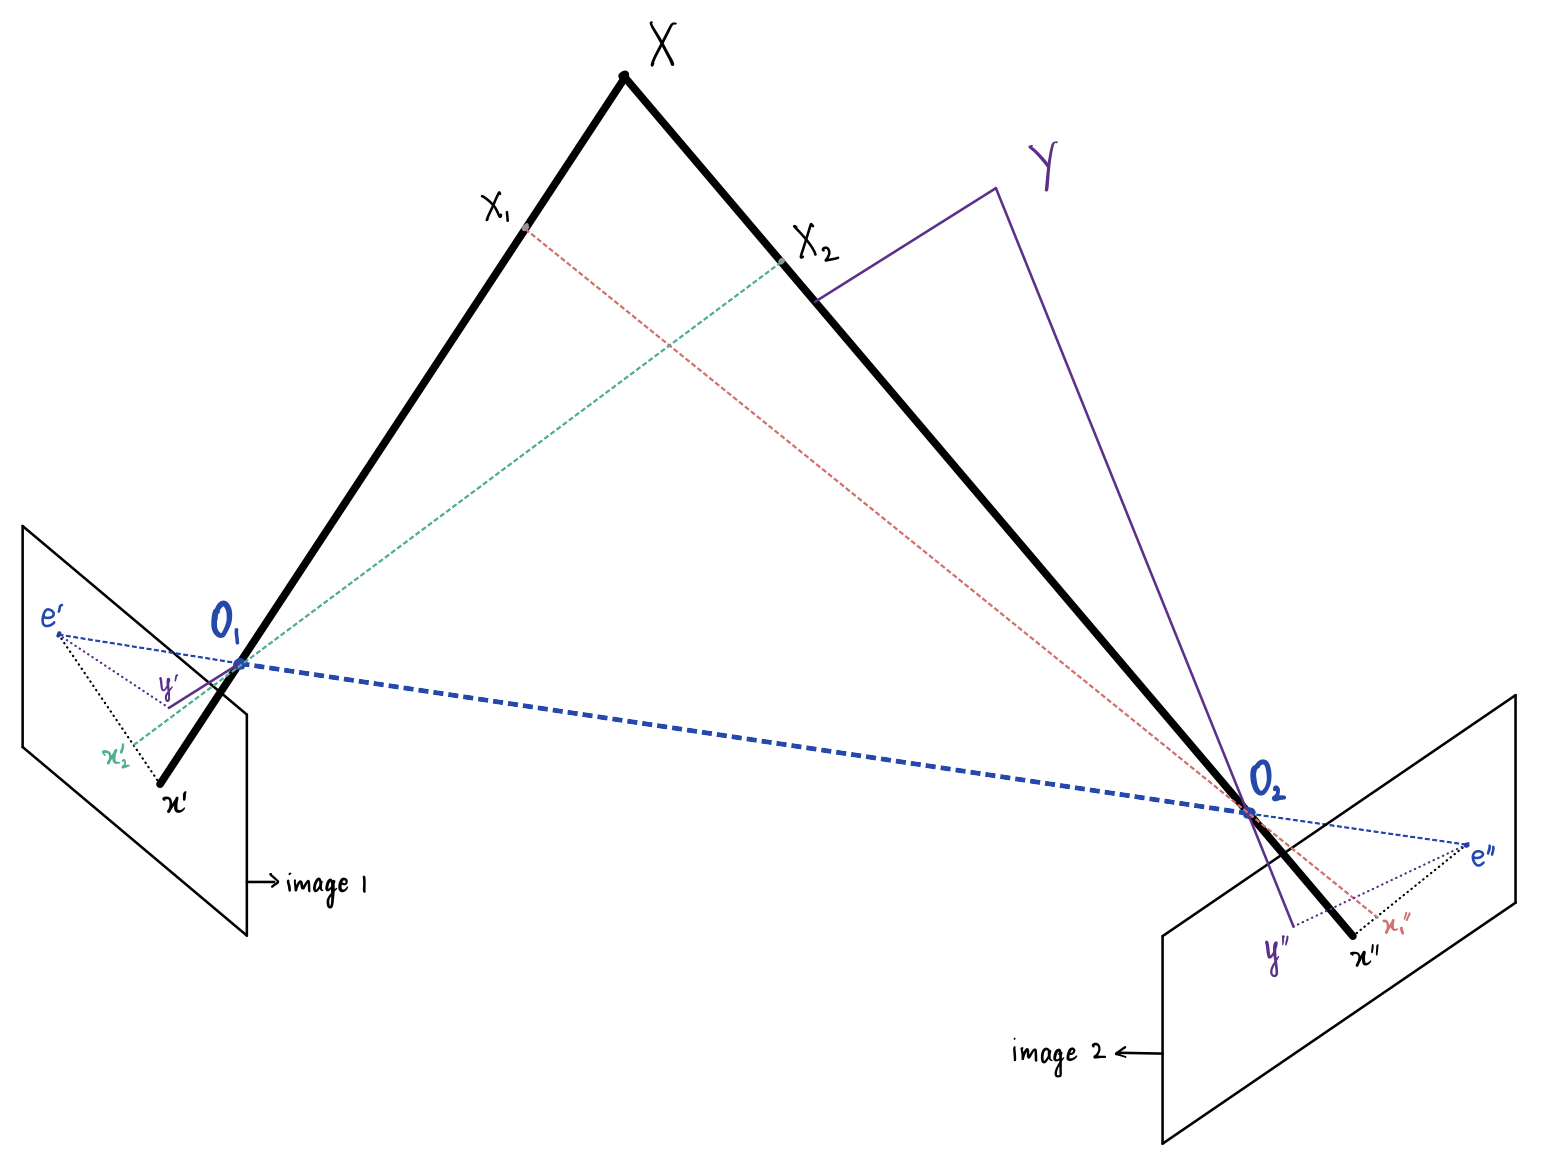
\includegraphics[width=0.6 \textwidth]{Epipolar_geometry.PNG}
    \caption{Epipolar Geometry}
    \label{fig:q1-epipolar-geometry}
    \small
        Points $X$ and $Y$ are points in the real world whose image falls at (pixel locations) $x'$ and $y'$ in image 1 and $x''$ and $y''$ in image 2. The origins of these cameras is located at $O_1$ and $O_2$ respectively. The line joining $O_1$ and $O_2$ is called the \textbf{epipolar axis}. It intersects the images at $e'$ and $e''$ respectively. \\
        It is clear that the image of $X_1$ in camera 1 will also fall on $x'$ (same line), similarly the image of $X_2$ in camera 2 will also fall on $x''$. However, the image of $X_1$ in camera 2 will fall at $x_1''$, which is on the line joining $x''$ and $e''$. This line is called the \textbf{epipolar line}. Similarly, the image of $X_2$ in camera 1 will fall at $x_2'$ (which is also on the line joining $e'$ and $x'$).
        When $X_1$ moves along $\overline{XO_1}$, its image $x''_1$ traces a line in the second image (the \textit{epoipolar line}). Same can be said for $X_2$ and the first image.
\end{figure}

Since $O_1 O_2 X$ form a plane (called the \textbf{epipolar plane}), the triple product of these three vectors will be zero, that is $\left \langle O_1 X \;\; O_1 O_2 \;\; O_2 X \right \rangle = \mathbf{0}$, where $\left \langle \vec{a} \;\; \vec{b} \;\; \vec{c} \right \rangle = \vec{a} \cdot \left ( \vec{b} \times \vec{c} \right )$ is the volume of the parallelepiped formed by the three vectors. From camera projection properties we can write

\begin{align}
    x' = \mathbf{K}' \mathbf{R}' \left [ \mathbf{I} \mid -\mathbf{X}_{O'} \right ] X
    &&
    x'' = \mathbf{K}'' \mathbf{R}'' \left [ \mathbf{I} \mid -\mathbf{X}_{O''} \right ] X
    \label{eq:q1-camera-projection}
\end{align}

Where $\mathbf{K}'$, $\mathbf{R}' \left [ \mathbf{I} \mid -\mathbf{X}_{O'} \right ]$ and $\mathbf{K}''$, $\mathbf{R}'' \left [ \mathbf{I} \mid -\mathbf{X}_{O''} \right ]$ are camera intrinsic and extrinsic parameters (for camera 1 and camera 2) respectively. Note that all the above terms are in \textit{homogeneous coordinates}. The vector $X$ can be assumed to be unit-scale.

We know that $\overrightarrow{O_1 X} = X - X_{O'} \equiv \mathbf{R}'^{-1} \mathbf{K}'^{-1} x'$ and $\overrightarrow{O_2 X} = X - X_{O''} \equiv \mathbf{R}''^{-1} \mathbf{K}''^{-1} x''$. Another reduction is $\overrightarrow{O_1 O_2} = b$ for the baseline vector (joining the two camera centers). Therefore, the triple product constraint mentioned above can be reduced to

\begin{align}
    \left \langle O_1 X \;\; O_1 O_2 \;\; O_2 X \right \rangle = \mathbf{0}
    \Rightarrow \left ( X - X_{O'} \right ) \cdot \left ( b \times \left ( X - X_{O''} \right ) \right ) 
    \equiv \left ( \mathbf{R}'^{-1} \mathbf{K}'^{-1} x' \right ) \cdot \left ( b \times \left ( \mathbf{R}''^{-1} \mathbf{K}''^{-1} x'' \right ) \right ) = 0
    \nonumber
\end{align}

Using $a \cdot b = a^\top b$ and $a \times b = \left [ a \right ]_\times b$ (wehre $\left [ a \right ]_\times$ is the cross product skew symmetric matrix), we can reduce the above equation to

\begin{align}
    \left \langle O_1 X \;\; O_1 O_2 \;\; O_2 X \right \rangle =& \left ( \mathbf{R}'^{-1} \mathbf{K}'^{-1} x' \right ) \cdot \left ( b \times \left ( \mathbf{R}''^{-1} \mathbf{K}''^{-1} x'' \right ) \right ) =
        \left ( \mathbf{R}'^{-1} \mathbf{K}'^{-1} x' \right )^\top \left [ b \right ]_\times \left ( \mathbf{R}''^{-1} \mathbf{K}''^{-1} x'' \right )
    \nonumber \\
    =& x'^\top \left ( \mathbf{K}'^{-\top} \mathbf{R}'^{-\top} \left [ b \right ]_\times \mathbf{R}''^{-1} \mathbf{K}''^{-1} \right ) x'' = x'^\top \mathbf{F} x'' = 0
    \label{eq:q1-fmat-eq}
\end{align}

The equation \ref{eq:q1-fmat-eq} is the basis for two points (in different images) to be projected to the same point in the 3D world. Note that if the points correspond, then they satisfy the equation. This is not true the other way round as we'll see later.

% Asnwer for 1.a: Epipole condition
\subfile{q1a.tex}

% Answer for 1.b: Fundamental Matrix transpose
\subfile{q1b.tex}

% Answer for 1.c: Fundamental and Essential Matrix
\subfile{q1c.tex}
